% Created by tikzDevice version 0.10.1 on 2016-08-14 13:48:20
% !TEX encoding = UTF-8 Unicode
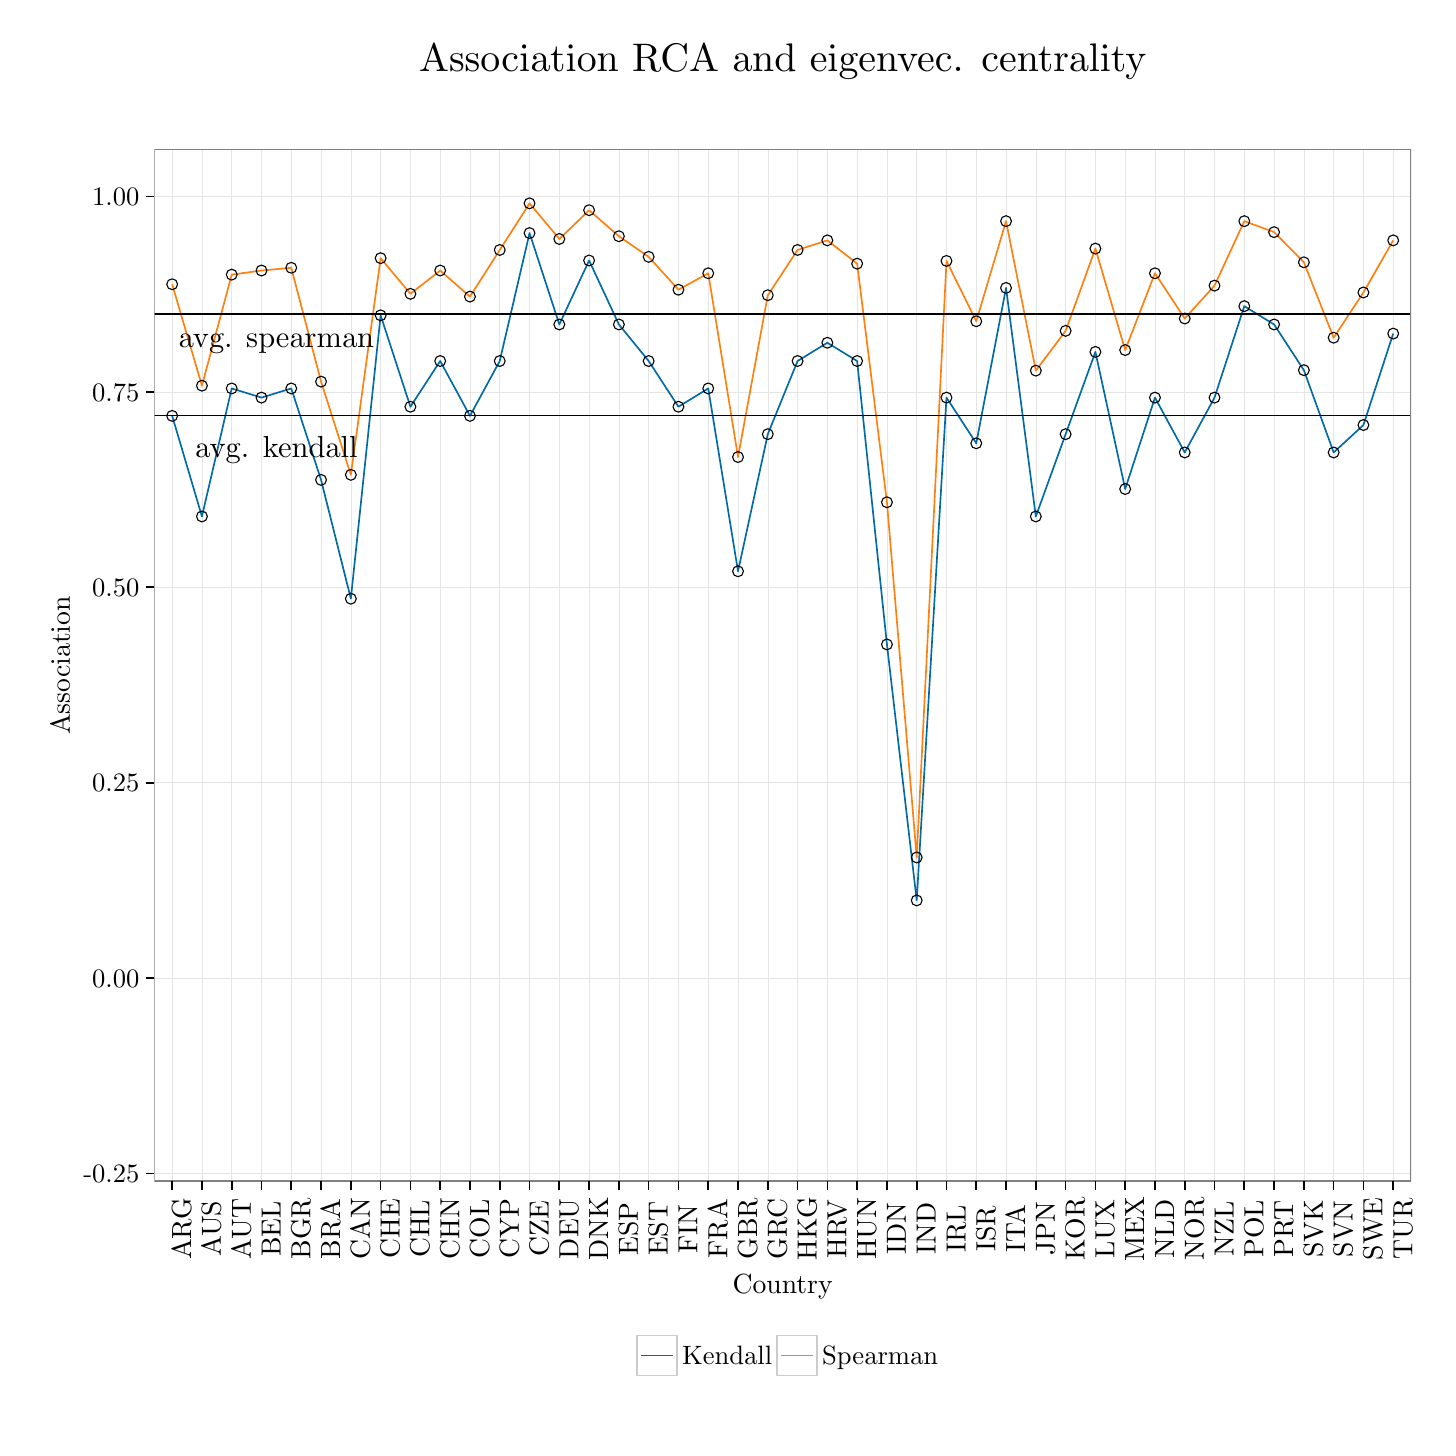
\begin{tikzpicture}[x=1pt,y=1pt]
\definecolor{fillColor}{RGB}{255,255,255}
\path[use as bounding box,fill=fillColor,fill opacity=0.00] (0,0) rectangle (505.89,505.89);
\begin{scope}
\path[clip] (  0.00,  0.00) rectangle (505.89,505.89);
\definecolor{drawColor}{RGB}{255,255,255}
\definecolor{fillColor}{RGB}{255,255,255}

\path[draw=drawColor,line width= 0.6pt,line join=round,line cap=round,fill=fillColor] (  0.00, -0.00) rectangle (505.89,505.89);
\end{scope}
\begin{scope}
\path[clip] ( 45.75, 89.02) rectangle (499.89,461.83);
\definecolor{fillColor}{RGB}{255,255,255}

\path[fill=fillColor] ( 45.75, 89.02) rectangle (499.89,461.83);
\definecolor{drawColor}{gray}{0.90}

\path[draw=drawColor,line width= 0.2pt,line join=round] ( 45.75, 91.84) --
	(499.89, 91.84);

\path[draw=drawColor,line width= 0.2pt,line join=round] ( 45.75,162.45) --
	(499.89,162.45);

\path[draw=drawColor,line width= 0.2pt,line join=round] ( 45.75,233.06) --
	(499.89,233.06);

\path[draw=drawColor,line width= 0.2pt,line join=round] ( 45.75,303.67) --
	(499.89,303.67);

\path[draw=drawColor,line width= 0.2pt,line join=round] ( 45.75,374.28) --
	(499.89,374.28);

\path[draw=drawColor,line width= 0.2pt,line join=round] ( 45.75,444.89) --
	(499.89,444.89);

\path[draw=drawColor,line width= 0.2pt,line join=round] ( 52.21, 89.02) --
	( 52.21,461.83);

\path[draw=drawColor,line width= 0.2pt,line join=round] ( 62.97, 89.02) --
	( 62.97,461.83);

\path[draw=drawColor,line width= 0.2pt,line join=round] ( 73.73, 89.02) --
	( 73.73,461.83);

\path[draw=drawColor,line width= 0.2pt,line join=round] ( 84.49, 89.02) --
	( 84.49,461.83);

\path[draw=drawColor,line width= 0.2pt,line join=round] ( 95.25, 89.02) --
	( 95.25,461.83);

\path[draw=drawColor,line width= 0.2pt,line join=round] (106.01, 89.02) --
	(106.01,461.83);

\path[draw=drawColor,line width= 0.2pt,line join=round] (116.78, 89.02) --
	(116.78,461.83);

\path[draw=drawColor,line width= 0.2pt,line join=round] (127.54, 89.02) --
	(127.54,461.83);

\path[draw=drawColor,line width= 0.2pt,line join=round] (138.30, 89.02) --
	(138.30,461.83);

\path[draw=drawColor,line width= 0.2pt,line join=round] (149.06, 89.02) --
	(149.06,461.83);

\path[draw=drawColor,line width= 0.2pt,line join=round] (159.82, 89.02) --
	(159.82,461.83);

\path[draw=drawColor,line width= 0.2pt,line join=round] (170.58, 89.02) --
	(170.58,461.83);

\path[draw=drawColor,line width= 0.2pt,line join=round] (181.35, 89.02) --
	(181.35,461.83);

\path[draw=drawColor,line width= 0.2pt,line join=round] (192.11, 89.02) --
	(192.11,461.83);

\path[draw=drawColor,line width= 0.2pt,line join=round] (202.87, 89.02) --
	(202.87,461.83);

\path[draw=drawColor,line width= 0.2pt,line join=round] (213.63, 89.02) --
	(213.63,461.83);

\path[draw=drawColor,line width= 0.2pt,line join=round] (224.39, 89.02) --
	(224.39,461.83);

\path[draw=drawColor,line width= 0.2pt,line join=round] (235.15, 89.02) --
	(235.15,461.83);

\path[draw=drawColor,line width= 0.2pt,line join=round] (245.92, 89.02) --
	(245.92,461.83);

\path[draw=drawColor,line width= 0.2pt,line join=round] (256.68, 89.02) --
	(256.68,461.83);

\path[draw=drawColor,line width= 0.2pt,line join=round] (267.44, 89.02) --
	(267.44,461.83);

\path[draw=drawColor,line width= 0.2pt,line join=round] (278.20, 89.02) --
	(278.20,461.83);

\path[draw=drawColor,line width= 0.2pt,line join=round] (288.96, 89.02) --
	(288.96,461.83);

\path[draw=drawColor,line width= 0.2pt,line join=round] (299.72, 89.02) --
	(299.72,461.83);

\path[draw=drawColor,line width= 0.2pt,line join=round] (310.49, 89.02) --
	(310.49,461.83);

\path[draw=drawColor,line width= 0.2pt,line join=round] (321.25, 89.02) --
	(321.25,461.83);

\path[draw=drawColor,line width= 0.2pt,line join=round] (332.01, 89.02) --
	(332.01,461.83);

\path[draw=drawColor,line width= 0.2pt,line join=round] (342.77, 89.02) --
	(342.77,461.83);

\path[draw=drawColor,line width= 0.2pt,line join=round] (353.53, 89.02) --
	(353.53,461.83);

\path[draw=drawColor,line width= 0.2pt,line join=round] (364.29, 89.02) --
	(364.29,461.83);

\path[draw=drawColor,line width= 0.2pt,line join=round] (375.06, 89.02) --
	(375.06,461.83);

\path[draw=drawColor,line width= 0.2pt,line join=round] (385.82, 89.02) --
	(385.82,461.83);

\path[draw=drawColor,line width= 0.2pt,line join=round] (396.58, 89.02) --
	(396.58,461.83);

\path[draw=drawColor,line width= 0.2pt,line join=round] (407.34, 89.02) --
	(407.34,461.83);

\path[draw=drawColor,line width= 0.2pt,line join=round] (418.10, 89.02) --
	(418.10,461.83);

\path[draw=drawColor,line width= 0.2pt,line join=round] (428.86, 89.02) --
	(428.86,461.83);

\path[draw=drawColor,line width= 0.2pt,line join=round] (439.62, 89.02) --
	(439.62,461.83);

\path[draw=drawColor,line width= 0.2pt,line join=round] (450.39, 89.02) --
	(450.39,461.83);

\path[draw=drawColor,line width= 0.2pt,line join=round] (461.15, 89.02) --
	(461.15,461.83);

\path[draw=drawColor,line width= 0.2pt,line join=round] (471.91, 89.02) --
	(471.91,461.83);

\path[draw=drawColor,line width= 0.2pt,line join=round] (482.67, 89.02) --
	(482.67,461.83);

\path[draw=drawColor,line width= 0.2pt,line join=round] (493.43, 89.02) --
	(493.43,461.83);
\definecolor{drawColor}{RGB}{0,107,164}

\path[draw=drawColor,line width= 0.6pt,line join=round] ( 52.21,365.61) --
	( 62.97,329.27) --
	( 73.73,375.52) --
	( 84.49,372.21) --
	( 95.25,375.52) --
	(106.01,342.48) --
	(116.78,299.54) --
	(127.54,401.94) --
	(138.30,368.91) --
	(149.06,385.43) --
	(159.82,365.61) --
	(170.58,385.43) --
	(181.35,431.67) --
	(192.11,398.64) --
	(202.87,421.76) --
	(213.63,398.64) --
	(224.39,385.43) --
	(235.15,368.91) --
	(245.92,375.52) --
	(256.68,309.45) --
	(267.44,359.00) --
	(278.20,385.43) --
	(288.96,392.03) --
	(299.72,385.43) --
	(310.49,283.02) --
	(321.25,190.53) --
	(332.01,372.21) --
	(342.77,355.70) --
	(353.53,411.85) --
	(364.29,329.27) --
	(375.06,359.00) --
	(385.82,388.73) --
	(396.58,339.18) --
	(407.34,372.21) --
	(418.10,352.39) --
	(428.86,372.21) --
	(439.62,405.25) --
	(450.39,398.64) --
	(461.15,382.12) --
	(471.91,352.39) --
	(482.67,362.30) --
	(493.43,395.34);
\definecolor{drawColor}{RGB}{255,128,14}

\path[draw=drawColor,line width= 0.6pt,line join=round] ( 52.21,413.17) --
	( 62.97,376.51) --
	( 73.73,416.64) --
	( 84.49,418.13) --
	( 95.25,419.12) --
	(106.01,377.99) --
	(116.78,344.30) --
	(127.54,422.59) --
	(138.30,409.71) --
	(149.06,418.13) --
	(159.82,408.71) --
	(170.58,425.56) --
	(181.35,442.41) --
	(192.11,429.53) --
	(202.87,439.93) --
	(213.63,430.52) --
	(224.39,423.08) --
	(235.15,411.19) --
	(245.92,417.14) --
	(256.68,350.74) --
	(267.44,409.21) --
	(278.20,425.56) --
	(288.96,429.03) --
	(299.72,420.61) --
	(310.49,334.39) --
	(321.25,206.05) --
	(332.01,421.60) --
	(342.77,399.80) --
	(353.53,435.97) --
	(364.29,381.96) --
	(375.06,396.33) --
	(385.82,426.06) --
	(396.58,389.39) --
	(407.34,417.14) --
	(418.10,400.79) --
	(428.86,412.68) --
	(439.62,435.97) --
	(450.39,432.00) --
	(461.15,421.10) --
	(471.91,393.85) --
	(482.67,410.20) --
	(493.43,429.03);
\definecolor{drawColor}{RGB}{0,0,0}

\path[draw=drawColor,line width= 0.4pt,line join=round,line cap=round] ( 52.21,365.61) circle (  1.96);

\path[draw=drawColor,line width= 0.4pt,line join=round,line cap=round] ( 62.97,329.27) circle (  1.96);

\path[draw=drawColor,line width= 0.4pt,line join=round,line cap=round] ( 73.73,375.52) circle (  1.96);

\path[draw=drawColor,line width= 0.4pt,line join=round,line cap=round] ( 84.49,372.21) circle (  1.96);

\path[draw=drawColor,line width= 0.4pt,line join=round,line cap=round] ( 95.25,375.52) circle (  1.96);

\path[draw=drawColor,line width= 0.4pt,line join=round,line cap=round] (106.01,342.48) circle (  1.96);

\path[draw=drawColor,line width= 0.4pt,line join=round,line cap=round] (116.78,299.54) circle (  1.96);

\path[draw=drawColor,line width= 0.4pt,line join=round,line cap=round] (127.54,401.94) circle (  1.96);

\path[draw=drawColor,line width= 0.4pt,line join=round,line cap=round] (138.30,368.91) circle (  1.96);

\path[draw=drawColor,line width= 0.4pt,line join=round,line cap=round] (149.06,385.43) circle (  1.96);

\path[draw=drawColor,line width= 0.4pt,line join=round,line cap=round] (159.82,365.61) circle (  1.96);

\path[draw=drawColor,line width= 0.4pt,line join=round,line cap=round] (170.58,385.43) circle (  1.96);

\path[draw=drawColor,line width= 0.4pt,line join=round,line cap=round] (181.35,431.67) circle (  1.96);

\path[draw=drawColor,line width= 0.4pt,line join=round,line cap=round] (192.11,398.64) circle (  1.96);

\path[draw=drawColor,line width= 0.4pt,line join=round,line cap=round] (202.87,421.76) circle (  1.96);

\path[draw=drawColor,line width= 0.4pt,line join=round,line cap=round] (213.63,398.64) circle (  1.96);

\path[draw=drawColor,line width= 0.4pt,line join=round,line cap=round] (224.39,385.43) circle (  1.96);

\path[draw=drawColor,line width= 0.4pt,line join=round,line cap=round] (235.15,368.91) circle (  1.96);

\path[draw=drawColor,line width= 0.4pt,line join=round,line cap=round] (245.92,375.52) circle (  1.96);

\path[draw=drawColor,line width= 0.4pt,line join=round,line cap=round] (256.68,309.45) circle (  1.96);

\path[draw=drawColor,line width= 0.4pt,line join=round,line cap=round] (267.44,359.00) circle (  1.96);

\path[draw=drawColor,line width= 0.4pt,line join=round,line cap=round] (278.20,385.43) circle (  1.96);

\path[draw=drawColor,line width= 0.4pt,line join=round,line cap=round] (288.96,392.03) circle (  1.96);

\path[draw=drawColor,line width= 0.4pt,line join=round,line cap=round] (299.72,385.43) circle (  1.96);

\path[draw=drawColor,line width= 0.4pt,line join=round,line cap=round] (310.49,283.02) circle (  1.96);

\path[draw=drawColor,line width= 0.4pt,line join=round,line cap=round] (321.25,190.53) circle (  1.96);

\path[draw=drawColor,line width= 0.4pt,line join=round,line cap=round] (332.01,372.21) circle (  1.96);

\path[draw=drawColor,line width= 0.4pt,line join=round,line cap=round] (342.77,355.70) circle (  1.96);

\path[draw=drawColor,line width= 0.4pt,line join=round,line cap=round] (353.53,411.85) circle (  1.96);

\path[draw=drawColor,line width= 0.4pt,line join=round,line cap=round] (364.29,329.27) circle (  1.96);

\path[draw=drawColor,line width= 0.4pt,line join=round,line cap=round] (375.06,359.00) circle (  1.96);

\path[draw=drawColor,line width= 0.4pt,line join=round,line cap=round] (385.82,388.73) circle (  1.96);

\path[draw=drawColor,line width= 0.4pt,line join=round,line cap=round] (396.58,339.18) circle (  1.96);

\path[draw=drawColor,line width= 0.4pt,line join=round,line cap=round] (407.34,372.21) circle (  1.96);

\path[draw=drawColor,line width= 0.4pt,line join=round,line cap=round] (418.10,352.39) circle (  1.96);

\path[draw=drawColor,line width= 0.4pt,line join=round,line cap=round] (428.86,372.21) circle (  1.96);

\path[draw=drawColor,line width= 0.4pt,line join=round,line cap=round] (439.62,405.25) circle (  1.96);

\path[draw=drawColor,line width= 0.4pt,line join=round,line cap=round] (450.39,398.64) circle (  1.96);

\path[draw=drawColor,line width= 0.4pt,line join=round,line cap=round] (461.15,382.12) circle (  1.96);

\path[draw=drawColor,line width= 0.4pt,line join=round,line cap=round] (471.91,352.39) circle (  1.96);

\path[draw=drawColor,line width= 0.4pt,line join=round,line cap=round] (482.67,362.30) circle (  1.96);

\path[draw=drawColor,line width= 0.4pt,line join=round,line cap=round] (493.43,395.34) circle (  1.96);

\path[draw=drawColor,line width= 0.4pt,line join=round,line cap=round] ( 52.21,413.17) circle (  1.96);

\path[draw=drawColor,line width= 0.4pt,line join=round,line cap=round] ( 62.97,376.51) circle (  1.96);

\path[draw=drawColor,line width= 0.4pt,line join=round,line cap=round] ( 73.73,416.64) circle (  1.96);

\path[draw=drawColor,line width= 0.4pt,line join=round,line cap=round] ( 84.49,418.13) circle (  1.96);

\path[draw=drawColor,line width= 0.4pt,line join=round,line cap=round] ( 95.25,419.12) circle (  1.96);

\path[draw=drawColor,line width= 0.4pt,line join=round,line cap=round] (106.01,377.99) circle (  1.96);

\path[draw=drawColor,line width= 0.4pt,line join=round,line cap=round] (116.78,344.30) circle (  1.96);

\path[draw=drawColor,line width= 0.4pt,line join=round,line cap=round] (127.54,422.59) circle (  1.96);

\path[draw=drawColor,line width= 0.4pt,line join=round,line cap=round] (138.30,409.71) circle (  1.96);

\path[draw=drawColor,line width= 0.4pt,line join=round,line cap=round] (149.06,418.13) circle (  1.96);

\path[draw=drawColor,line width= 0.4pt,line join=round,line cap=round] (159.82,408.71) circle (  1.96);

\path[draw=drawColor,line width= 0.4pt,line join=round,line cap=round] (170.58,425.56) circle (  1.96);

\path[draw=drawColor,line width= 0.4pt,line join=round,line cap=round] (181.35,442.41) circle (  1.96);

\path[draw=drawColor,line width= 0.4pt,line join=round,line cap=round] (192.11,429.53) circle (  1.96);

\path[draw=drawColor,line width= 0.4pt,line join=round,line cap=round] (202.87,439.93) circle (  1.96);

\path[draw=drawColor,line width= 0.4pt,line join=round,line cap=round] (213.63,430.52) circle (  1.96);

\path[draw=drawColor,line width= 0.4pt,line join=round,line cap=round] (224.39,423.08) circle (  1.96);

\path[draw=drawColor,line width= 0.4pt,line join=round,line cap=round] (235.15,411.19) circle (  1.96);

\path[draw=drawColor,line width= 0.4pt,line join=round,line cap=round] (245.92,417.14) circle (  1.96);

\path[draw=drawColor,line width= 0.4pt,line join=round,line cap=round] (256.68,350.74) circle (  1.96);

\path[draw=drawColor,line width= 0.4pt,line join=round,line cap=round] (267.44,409.21) circle (  1.96);

\path[draw=drawColor,line width= 0.4pt,line join=round,line cap=round] (278.20,425.56) circle (  1.96);

\path[draw=drawColor,line width= 0.4pt,line join=round,line cap=round] (288.96,429.03) circle (  1.96);

\path[draw=drawColor,line width= 0.4pt,line join=round,line cap=round] (299.72,420.61) circle (  1.96);

\path[draw=drawColor,line width= 0.4pt,line join=round,line cap=round] (310.49,334.39) circle (  1.96);

\path[draw=drawColor,line width= 0.4pt,line join=round,line cap=round] (321.25,206.05) circle (  1.96);

\path[draw=drawColor,line width= 0.4pt,line join=round,line cap=round] (332.01,421.60) circle (  1.96);

\path[draw=drawColor,line width= 0.4pt,line join=round,line cap=round] (342.77,399.80) circle (  1.96);

\path[draw=drawColor,line width= 0.4pt,line join=round,line cap=round] (353.53,435.97) circle (  1.96);

\path[draw=drawColor,line width= 0.4pt,line join=round,line cap=round] (364.29,381.96) circle (  1.96);

\path[draw=drawColor,line width= 0.4pt,line join=round,line cap=round] (375.06,396.33) circle (  1.96);

\path[draw=drawColor,line width= 0.4pt,line join=round,line cap=round] (385.82,426.06) circle (  1.96);

\path[draw=drawColor,line width= 0.4pt,line join=round,line cap=round] (396.58,389.39) circle (  1.96);

\path[draw=drawColor,line width= 0.4pt,line join=round,line cap=round] (407.34,417.14) circle (  1.96);

\path[draw=drawColor,line width= 0.4pt,line join=round,line cap=round] (418.10,400.79) circle (  1.96);

\path[draw=drawColor,line width= 0.4pt,line join=round,line cap=round] (428.86,412.68) circle (  1.96);

\path[draw=drawColor,line width= 0.4pt,line join=round,line cap=round] (439.62,435.97) circle (  1.96);

\path[draw=drawColor,line width= 0.4pt,line join=round,line cap=round] (450.39,432.00) circle (  1.96);

\path[draw=drawColor,line width= 0.4pt,line join=round,line cap=round] (461.15,421.10) circle (  1.96);

\path[draw=drawColor,line width= 0.4pt,line join=round,line cap=round] (471.91,393.85) circle (  1.96);

\path[draw=drawColor,line width= 0.4pt,line join=round,line cap=round] (482.67,410.20) circle (  1.96);

\path[draw=drawColor,line width= 0.4pt,line join=round,line cap=round] (493.43,429.03) circle (  1.96);

\path[draw=drawColor,line width= 0.6pt,line join=round] ( 45.75,402.52) -- (499.89,402.52);

\node[text=drawColor,anchor=base,inner sep=0pt, outer sep=0pt, scale=  1.10] at ( 89.87,390.25) {avg. spearman};

\path[draw=drawColor,line width= 0.6pt,line join=round] ( 45.75,365.80) -- (499.89,365.80);

\node[text=drawColor,anchor=base,inner sep=0pt, outer sep=0pt, scale=  1.10] at ( 89.87,350.70) {avg. kendall};
\definecolor{drawColor}{gray}{0.50}

\path[draw=drawColor,line width= 0.6pt,line join=round,line cap=round] ( 45.75, 89.02) rectangle (499.89,461.83);
\end{scope}
\begin{scope}
\path[clip] (  0.00,  0.00) rectangle (505.89,505.89);
\definecolor{drawColor}{RGB}{0,0,0}

\node[text=drawColor,anchor=base east,inner sep=0pt, outer sep=0pt, scale=  0.96] at ( 40.35, 88.53) {-0.25};

\node[text=drawColor,anchor=base east,inner sep=0pt, outer sep=0pt, scale=  0.96] at ( 40.35,159.14) {0.00};

\node[text=drawColor,anchor=base east,inner sep=0pt, outer sep=0pt, scale=  0.96] at ( 40.35,229.75) {0.25};

\node[text=drawColor,anchor=base east,inner sep=0pt, outer sep=0pt, scale=  0.96] at ( 40.35,300.36) {0.50};

\node[text=drawColor,anchor=base east,inner sep=0pt, outer sep=0pt, scale=  0.96] at ( 40.35,370.97) {0.75};

\node[text=drawColor,anchor=base east,inner sep=0pt, outer sep=0pt, scale=  0.96] at ( 40.35,441.58) {1.00};
\end{scope}
\begin{scope}
\path[clip] (  0.00,  0.00) rectangle (505.89,505.89);
\definecolor{drawColor}{RGB}{0,0,0}

\path[draw=drawColor,line width= 0.6pt,line join=round] ( 42.75, 91.84) --
	( 45.75, 91.84);

\path[draw=drawColor,line width= 0.6pt,line join=round] ( 42.75,162.45) --
	( 45.75,162.45);

\path[draw=drawColor,line width= 0.6pt,line join=round] ( 42.75,233.06) --
	( 45.75,233.06);

\path[draw=drawColor,line width= 0.6pt,line join=round] ( 42.75,303.67) --
	( 45.75,303.67);

\path[draw=drawColor,line width= 0.6pt,line join=round] ( 42.75,374.28) --
	( 45.75,374.28);

\path[draw=drawColor,line width= 0.6pt,line join=round] ( 42.75,444.89) --
	( 45.75,444.89);
\end{scope}
\begin{scope}
\path[clip] (  0.00,  0.00) rectangle (505.89,505.89);
\definecolor{drawColor}{RGB}{0,0,0}

\path[draw=drawColor,line width= 0.6pt,line join=round] ( 52.21, 86.02) --
	( 52.21, 89.02);

\path[draw=drawColor,line width= 0.6pt,line join=round] ( 62.97, 86.02) --
	( 62.97, 89.02);

\path[draw=drawColor,line width= 0.6pt,line join=round] ( 73.73, 86.02) --
	( 73.73, 89.02);

\path[draw=drawColor,line width= 0.6pt,line join=round] ( 84.49, 86.02) --
	( 84.49, 89.02);

\path[draw=drawColor,line width= 0.6pt,line join=round] ( 95.25, 86.02) --
	( 95.25, 89.02);

\path[draw=drawColor,line width= 0.6pt,line join=round] (106.01, 86.02) --
	(106.01, 89.02);

\path[draw=drawColor,line width= 0.6pt,line join=round] (116.78, 86.02) --
	(116.78, 89.02);

\path[draw=drawColor,line width= 0.6pt,line join=round] (127.54, 86.02) --
	(127.54, 89.02);

\path[draw=drawColor,line width= 0.6pt,line join=round] (138.30, 86.02) --
	(138.30, 89.02);

\path[draw=drawColor,line width= 0.6pt,line join=round] (149.06, 86.02) --
	(149.06, 89.02);

\path[draw=drawColor,line width= 0.6pt,line join=round] (159.82, 86.02) --
	(159.82, 89.02);

\path[draw=drawColor,line width= 0.6pt,line join=round] (170.58, 86.02) --
	(170.58, 89.02);

\path[draw=drawColor,line width= 0.6pt,line join=round] (181.35, 86.02) --
	(181.35, 89.02);

\path[draw=drawColor,line width= 0.6pt,line join=round] (192.11, 86.02) --
	(192.11, 89.02);

\path[draw=drawColor,line width= 0.6pt,line join=round] (202.87, 86.02) --
	(202.87, 89.02);

\path[draw=drawColor,line width= 0.6pt,line join=round] (213.63, 86.02) --
	(213.63, 89.02);

\path[draw=drawColor,line width= 0.6pt,line join=round] (224.39, 86.02) --
	(224.39, 89.02);

\path[draw=drawColor,line width= 0.6pt,line join=round] (235.15, 86.02) --
	(235.15, 89.02);

\path[draw=drawColor,line width= 0.6pt,line join=round] (245.92, 86.02) --
	(245.92, 89.02);

\path[draw=drawColor,line width= 0.6pt,line join=round] (256.68, 86.02) --
	(256.68, 89.02);

\path[draw=drawColor,line width= 0.6pt,line join=round] (267.44, 86.02) --
	(267.44, 89.02);

\path[draw=drawColor,line width= 0.6pt,line join=round] (278.20, 86.02) --
	(278.20, 89.02);

\path[draw=drawColor,line width= 0.6pt,line join=round] (288.96, 86.02) --
	(288.96, 89.02);

\path[draw=drawColor,line width= 0.6pt,line join=round] (299.72, 86.02) --
	(299.72, 89.02);

\path[draw=drawColor,line width= 0.6pt,line join=round] (310.49, 86.02) --
	(310.49, 89.02);

\path[draw=drawColor,line width= 0.6pt,line join=round] (321.25, 86.02) --
	(321.25, 89.02);

\path[draw=drawColor,line width= 0.6pt,line join=round] (332.01, 86.02) --
	(332.01, 89.02);

\path[draw=drawColor,line width= 0.6pt,line join=round] (342.77, 86.02) --
	(342.77, 89.02);

\path[draw=drawColor,line width= 0.6pt,line join=round] (353.53, 86.02) --
	(353.53, 89.02);

\path[draw=drawColor,line width= 0.6pt,line join=round] (364.29, 86.02) --
	(364.29, 89.02);

\path[draw=drawColor,line width= 0.6pt,line join=round] (375.06, 86.02) --
	(375.06, 89.02);

\path[draw=drawColor,line width= 0.6pt,line join=round] (385.82, 86.02) --
	(385.82, 89.02);

\path[draw=drawColor,line width= 0.6pt,line join=round] (396.58, 86.02) --
	(396.58, 89.02);

\path[draw=drawColor,line width= 0.6pt,line join=round] (407.34, 86.02) --
	(407.34, 89.02);

\path[draw=drawColor,line width= 0.6pt,line join=round] (418.10, 86.02) --
	(418.10, 89.02);

\path[draw=drawColor,line width= 0.6pt,line join=round] (428.86, 86.02) --
	(428.86, 89.02);

\path[draw=drawColor,line width= 0.6pt,line join=round] (439.62, 86.02) --
	(439.62, 89.02);

\path[draw=drawColor,line width= 0.6pt,line join=round] (450.39, 86.02) --
	(450.39, 89.02);

\path[draw=drawColor,line width= 0.6pt,line join=round] (461.15, 86.02) --
	(461.15, 89.02);

\path[draw=drawColor,line width= 0.6pt,line join=round] (471.91, 86.02) --
	(471.91, 89.02);

\path[draw=drawColor,line width= 0.6pt,line join=round] (482.67, 86.02) --
	(482.67, 89.02);

\path[draw=drawColor,line width= 0.6pt,line join=round] (493.43, 86.02) --
	(493.43, 89.02);
\end{scope}
\begin{scope}
\path[clip] (  0.00,  0.00) rectangle (505.89,505.89);
\definecolor{drawColor}{RGB}{0,0,0}

\node[text=drawColor,rotate= 90.00,anchor=base,inner sep=0pt, outer sep=0pt, scale=  1.00] at ( 59.09, 71.88) {ARG};

\node[text=drawColor,rotate= 90.00,anchor=base,inner sep=0pt, outer sep=0pt, scale=  1.00] at ( 69.85, 71.88) {AUS};

\node[text=drawColor,rotate= 90.00,anchor=base,inner sep=0pt, outer sep=0pt, scale=  1.00] at ( 80.62, 71.88) {AUT};

\node[text=drawColor,rotate= 90.00,anchor=base,inner sep=0pt, outer sep=0pt, scale=  1.00] at ( 91.38, 71.88) {BEL};

\node[text=drawColor,rotate= 90.00,anchor=base,inner sep=0pt, outer sep=0pt, scale=  1.00] at (102.14, 71.88) {BGR};

\node[text=drawColor,rotate= 90.00,anchor=base,inner sep=0pt, outer sep=0pt, scale=  1.00] at (112.90, 71.88) {BRA};

\node[text=drawColor,rotate= 90.00,anchor=base,inner sep=0pt, outer sep=0pt, scale=  1.00] at (123.66, 71.88) {CAN};

\node[text=drawColor,rotate= 90.00,anchor=base,inner sep=0pt, outer sep=0pt, scale=  1.00] at (134.42, 71.88) {CHE};

\node[text=drawColor,rotate= 90.00,anchor=base,inner sep=0pt, outer sep=0pt, scale=  1.00] at (145.19, 71.88) {CHL};

\node[text=drawColor,rotate= 90.00,anchor=base,inner sep=0pt, outer sep=0pt, scale=  1.00] at (155.95, 71.88) {CHN};

\node[text=drawColor,rotate= 90.00,anchor=base,inner sep=0pt, outer sep=0pt, scale=  1.00] at (166.71, 71.88) {COL};

\node[text=drawColor,rotate= 90.00,anchor=base,inner sep=0pt, outer sep=0pt, scale=  1.00] at (177.47, 71.88) {CYP};

\node[text=drawColor,rotate= 90.00,anchor=base,inner sep=0pt, outer sep=0pt, scale=  1.00] at (188.23, 71.88) {CZE};

\node[text=drawColor,rotate= 90.00,anchor=base,inner sep=0pt, outer sep=0pt, scale=  1.00] at (198.99, 71.88) {DEU};

\node[text=drawColor,rotate= 90.00,anchor=base,inner sep=0pt, outer sep=0pt, scale=  1.00] at (209.76, 71.88) {DNK};

\node[text=drawColor,rotate= 90.00,anchor=base,inner sep=0pt, outer sep=0pt, scale=  1.00] at (220.52, 71.88) {ESP};

\node[text=drawColor,rotate= 90.00,anchor=base,inner sep=0pt, outer sep=0pt, scale=  1.00] at (231.28, 71.88) {EST};

\node[text=drawColor,rotate= 90.00,anchor=base,inner sep=0pt, outer sep=0pt, scale=  1.00] at (242.04, 71.88) {FIN};

\node[text=drawColor,rotate= 90.00,anchor=base,inner sep=0pt, outer sep=0pt, scale=  1.00] at (252.80, 71.88) {FRA};

\node[text=drawColor,rotate= 90.00,anchor=base,inner sep=0pt, outer sep=0pt, scale=  1.00] at (263.56, 71.88) {GBR};

\node[text=drawColor,rotate= 90.00,anchor=base,inner sep=0pt, outer sep=0pt, scale=  1.00] at (274.33, 71.88) {GRC};

\node[text=drawColor,rotate= 90.00,anchor=base,inner sep=0pt, outer sep=0pt, scale=  1.00] at (285.09, 71.88) {HKG};

\node[text=drawColor,rotate= 90.00,anchor=base,inner sep=0pt, outer sep=0pt, scale=  1.00] at (295.85, 71.88) {HRV};

\node[text=drawColor,rotate= 90.00,anchor=base,inner sep=0pt, outer sep=0pt, scale=  1.00] at (306.61, 71.88) {HUN};

\node[text=drawColor,rotate= 90.00,anchor=base,inner sep=0pt, outer sep=0pt, scale=  1.00] at (317.37, 71.88) {IDN};

\node[text=drawColor,rotate= 90.00,anchor=base,inner sep=0pt, outer sep=0pt, scale=  1.00] at (328.13, 71.88) {IND};

\node[text=drawColor,rotate= 90.00,anchor=base,inner sep=0pt, outer sep=0pt, scale=  1.00] at (338.90, 71.88) {IRL};

\node[text=drawColor,rotate= 90.00,anchor=base,inner sep=0pt, outer sep=0pt, scale=  1.00] at (349.66, 71.88) {ISR};

\node[text=drawColor,rotate= 90.00,anchor=base,inner sep=0pt, outer sep=0pt, scale=  1.00] at (360.42, 71.88) {ITA};

\node[text=drawColor,rotate= 90.00,anchor=base,inner sep=0pt, outer sep=0pt, scale=  1.00] at (371.18, 71.88) {JPN};

\node[text=drawColor,rotate= 90.00,anchor=base,inner sep=0pt, outer sep=0pt, scale=  1.00] at (381.94, 71.88) {KOR};

\node[text=drawColor,rotate= 90.00,anchor=base,inner sep=0pt, outer sep=0pt, scale=  1.00] at (392.70, 71.88) {LUX};

\node[text=drawColor,rotate= 90.00,anchor=base,inner sep=0pt, outer sep=0pt, scale=  1.00] at (403.47, 71.88) {MEX};

\node[text=drawColor,rotate= 90.00,anchor=base,inner sep=0pt, outer sep=0pt, scale=  1.00] at (414.23, 71.88) {NLD};

\node[text=drawColor,rotate= 90.00,anchor=base,inner sep=0pt, outer sep=0pt, scale=  1.00] at (424.99, 71.88) {NOR};

\node[text=drawColor,rotate= 90.00,anchor=base,inner sep=0pt, outer sep=0pt, scale=  1.00] at (435.75, 71.88) {NZL};

\node[text=drawColor,rotate= 90.00,anchor=base,inner sep=0pt, outer sep=0pt, scale=  1.00] at (446.51, 71.88) {POL};

\node[text=drawColor,rotate= 90.00,anchor=base,inner sep=0pt, outer sep=0pt, scale=  1.00] at (457.27, 71.88) {PRT};

\node[text=drawColor,rotate= 90.00,anchor=base,inner sep=0pt, outer sep=0pt, scale=  1.00] at (468.04, 71.88) {SVK};

\node[text=drawColor,rotate= 90.00,anchor=base,inner sep=0pt, outer sep=0pt, scale=  1.00] at (478.80, 71.88) {SVN};

\node[text=drawColor,rotate= 90.00,anchor=base,inner sep=0pt, outer sep=0pt, scale=  1.00] at (489.56, 71.88) {SWE};

\node[text=drawColor,rotate= 90.00,anchor=base,inner sep=0pt, outer sep=0pt, scale=  1.00] at (500.32, 71.88) {TUR};
\end{scope}
\begin{scope}
\path[clip] (  0.00,  0.00) rectangle (505.89,505.89);
\definecolor{drawColor}{RGB}{0,0,0}

\node[text=drawColor,anchor=base,inner sep=0pt, outer sep=0pt, scale=  1.00] at (272.82, 48.46) {Country};
\end{scope}
\begin{scope}
\path[clip] (  0.00,  0.00) rectangle (505.89,505.89);
\definecolor{drawColor}{RGB}{0,0,0}

\node[text=drawColor,rotate= 90.00,anchor=base,inner sep=0pt, outer sep=0pt, scale=  1.00] at ( 15.29,275.42) {Association};
\end{scope}
\begin{scope}
\path[clip] (  0.00,  0.00) rectangle (505.89,505.89);
\definecolor{fillColor}{RGB}{255,255,255}

\path[fill=fillColor] (212.38, 14.54) rectangle (333.26, 37.53);
\end{scope}
\begin{scope}
\path[clip] (  0.00,  0.00) rectangle (505.89,505.89);
\definecolor{drawColor}{gray}{0.80}
\definecolor{fillColor}{RGB}{255,255,255}

\path[draw=drawColor,line width= 0.6pt,line join=round,line cap=round,fill=fillColor] (220.26, 18.80) rectangle (234.71, 33.26);
\end{scope}
\begin{scope}
\path[clip] (  0.00,  0.00) rectangle (505.89,505.89);
\definecolor{drawColor}{RGB}{0,107,164}

\path[draw=drawColor,line width= 0.6pt,line join=round] (221.70, 26.03) -- (233.27, 26.03);
\end{scope}
\begin{scope}
\path[clip] (  0.00,  0.00) rectangle (505.89,505.89);
\definecolor{drawColor}{gray}{0.80}
\definecolor{fillColor}{RGB}{255,255,255}

\path[draw=drawColor,line width= 0.6pt,line join=round,line cap=round,fill=fillColor] (270.85, 18.80) rectangle (285.30, 33.26);
\end{scope}
\begin{scope}
\path[clip] (  0.00,  0.00) rectangle (505.89,505.89);
\definecolor{drawColor}{RGB}{255,128,14}

\path[draw=drawColor,line width= 0.6pt,line join=round] (272.30, 26.03) -- (283.86, 26.03);
\end{scope}
\begin{scope}
\path[clip] (  0.00,  0.00) rectangle (505.89,505.89);
\definecolor{drawColor}{RGB}{0,0,0}

\node[text=drawColor,anchor=base west,inner sep=0pt, outer sep=0pt, scale=  0.96] at (236.52, 22.72) {Kendall};
\end{scope}
\begin{scope}
\path[clip] (  0.00,  0.00) rectangle (505.89,505.89);
\definecolor{drawColor}{RGB}{0,0,0}

\node[text=drawColor,anchor=base west,inner sep=0pt, outer sep=0pt, scale=  0.96] at (287.11, 22.72) {Spearman};
\end{scope}
\begin{scope}
\path[clip] (  0.00,  0.00) rectangle (505.89,505.89);
\definecolor{drawColor}{RGB}{0,0,0}

\node[text=drawColor,anchor=base west,inner sep=0pt, outer sep=0pt, scale=  1.44] at (141.45,489.97) {Association RCA and eigenvec. centrality};
\end{scope}
\end{tikzpicture}
